\chapter{设备管理}

\section{I/O重定向}

\subsection{标准I/O}

程序对读入的数据进行处理,再输出数据。数据的输入(input)和输出(output)简称为I/O,在没有指定输入输出的情况下,默认为标准输入和标准输出。 \\

打开的文件都有一个文件描述符(fd, file descriptor),表现为一个数字:

\begin{itemize}
	\item 标准输入stdin(键盘):fd = 0
	\item 标准输出stdout(显示器):fd = 1
	\item 标准错误输出stderr(显示器):fd = 2
\end{itemize}

\mybox{标准I/O}

\begin{lstlisting}[language=C]
#include <stdio.h>

int main(int argc, char *argv[]) {
    int num;
    printf("(stdin) enter an integer: ");
    fscanf(stdin, "%d", &num);
    fprintf(stdout, "(stdout) num = %d\n", num);
    fprintf(stderr, "(stderr) This is an error message.\n");
    return 0;
}
\end{lstlisting}

\begin{tcolorbox}
	\mybox{运行结果}
	\begin{verbatim}
(stdin) enter an integer: 123
(stdout) num = 123
(stderr) This is an error message.
	\end{verbatim}
\end{tcolorbox}

\vspace{0.5cm}

\mybox{文件I/O}

\begin{lstlisting}[language=C]
#include <stdio.h>
#include <stdlib.h>

void writeFile(const char *filename) {
    FILE *fp = fopen(filename, "w");
    if(!fp) {
        fprintf(stderr, "File open failed.\n");
        exit(1);
    }
    char *name = "小灰";
    int age = 17;
    double height = 182.3;
    fprintf(fp, "姓名:%s\n年龄:%d\n身高:%.2f\n", 
                name, age, height);
    fclose(fp);
}

void readFile(const char *filename) {
    FILE *fp = fopen(filename, "r");
    if(!fp) {
        fprintf(stderr, "File open failed.\n");
        exit(1);
    }
    char name[32];
    int age;
    double height;
    fscanf(fp, "姓名:%s\n年龄:%d\n身高:%lf\n", 
                name, &age, &height);
    printf("name: %s\n", name);
    printf("age: %d\n", age);
    printf("height: %.2f\n", height);
    fclose(fp);
}

int main(int argc, char *argv[]) {
    const char *filename = "info.txt";
    writeFile(filename);
    readFile(filename);
    return 0;
}
\end{lstlisting}

\begin{tcolorbox}
	\mybox{运行结果}
	\begin{verbatim}
name: 小灰
age: 17
height: 182.30
	\end{verbatim}
\end{tcolorbox}

\subsection{I/O重定向(I/O Redirection)}

I/O重定向就是改变标准输入与输出的默认位置。标准输入默认是键盘,通过改成其它输入,就是输入重定向,例如从文本文件里输入。标准输出默认是显示器,通过改成其它输出,就是输出重定向,例如输出到文件。 \\

输出重定向用【>】表示,若文件不存在,则创建;若文件已存在,则覆盖。使用【>>】时若文件不存在,则创建,若文件已存在,则追加。错误输出重定向用【2>】和【2>>】表示。 \\

输入重定向用【<】表示,但是在输入重定向中【<<】可不是表示输入追加。 \\

\mybox{I/O重定向}

\begin{lstlisting}[language=C]
#include <stdio.h>

int main(int argc, char *argv[]) {
    int data;
    scanf("%d", &data);
    printf("data = %d\n", data);
    return 0;
}
\end{lstlisting}

\begin{lstlisting}[title=input.txt]
12345
\end{lstlisting}

\begin{lstlisting}[title=编译]
gcc -Wall io_redirection.c -o io_redirection
\end{lstlisting}

\begin{lstlisting}[title=运行]
./io_redirection < input.txt > output.txt
\end{lstlisting}

\begin{tcolorbox}
	\mybox{运行结果}
	\textbf{output.txt}
	\begin{verbatim}
num = 12345
	\end{verbatim}
\end{tcolorbox}

\newpage

\section{I/O控制方式}

\subsection{I/O设备}

现代计算机系统总是配有各种类型的外部设备,除了显示器、键盘、打印机、磁带、磁盘外,又出现了光盘、绘图仪、图形数字化仪、鼠标器、激光打印机、声音输入输出设备等,种类繁多。不同外设之间的差异较大,因此I/O性能经常成为系统的瓶颈。 \\

操作系统设备管理的目标包括:

\begin{enumerate}
	\item 向用户提供使用外部设备的方便、统一的接口,按照用户的要求和设备的类型,控制设备工作,完成用户的输入输出请求。方便是指用户能独立于具体设备的复杂物理特性而方便地使用设备;统一是指对不同设备尽量能统一操作方式。方便和统一要求对用户屏蔽实现具体设备I/O操作的细节,呈现给用户的是一种性能理想化的、操作简便的逻辑设备。系统的这种性能亦称为设备的独立性(设备无关性)。

	\item 充分利用中断技术、通道技术和缓冲技术,提高CPU与设备、设备与设备间的并行工作能力,充分利用设备资源,提高外部设备的使用效率。

	\item 设备管理就是要保证在多道程序环境下,当多个进程竞争使用设备时,按照一定的策略分配和管理设备,以使系统能有条不紊地工作。
\end{enumerate}

\subsection{I/O控制方式}

早期,计算机设计者没有将CPU的执行与I/O操作分开,甚至大多数人认为输入输出与计算的时间应该是同一数量级。后来,他们意识到,CPU要比I/O操作速度高几个数量级。于是,硬件和软件设计师开始寻找一种技术,使CPU计算可以不用等待I/O操作而持续执行。 \\

I/O控制方式包括:

\begin{enumerate}
	\item 程序控制I/O(Programmed I/O):处理器代表一个进程给I/O模块发送一个I/O命令,该进程进入忙等待(busy waiting),直到操作完成。

	\item 中断驱动I/O(Interrupt I/O):处理器代表进程向I/O发送命令,如果来自进程的I/O指令是非阻塞的,那么处理器继续执行进程的后续指令。如果I/O指令时阻塞的,那么处理器执行来自操作系统的指令,将当前进程设置为阻塞态并且调度其它进程。

	\item 直接存储器访问(DMA):DMA模块控制内存和I/O模块之间的数据交换。为传送一块数据,处理器给DMA模块发送请求,只有当整个数据块传送结束后,它才能被中断。
\end{enumerate}

\newpage

\section{I/O缓冲}

\subsection{I/O缓冲(I/O Buffering)}

在设备管理中,为了缓和CPU与I/O设备速度不匹配的矛盾,提高CPU与I/O设备的并行性、减少对CPU的中断频率,在I/O设备与处理机交换数据时都用到了缓冲区。 \\

缓冲的种类包括:

\begin{enumerate}
	\item 单缓冲:输入时通道先将数据送入缓冲区,CPU从缓冲区取数据处理。通道再送入后续数据,如此反复直到输入完成。输出情形正好相反。由于缓冲区属于互斥区,所以单缓冲并不能明显改善CPU与外部设备的并行性。

	      \begin{figure}[H]
		      \centering
		      \begin{tikzpicture}[scale=0.7]
			      \draw[rounded corners] (0,0) rectangle (3,2);
			      \draw[rounded corners] (6,0) rectangle (9,2);
			      \draw[rounded corners] (12,0) rectangle (15,2);

			      \draw (1.5,1) node {外设};
			      \draw (7.5,1) node {缓冲区};
			      \draw (13.5,1) node {CPU};

			      \draw[->] (3,1) -- (6,1);
			      \draw[->] (9,1) -- (12,1);
		      \end{tikzpicture}
		      \caption{单缓冲}
	      \end{figure}

	\item 双缓冲:分别设置输入缓冲区和输出缓冲区,CPU和通道可以分别访问两个缓冲区,即在CPU访问一个缓冲区的同时,通道可以访问另一个缓冲区。双缓冲只是一种说明设备和设备、CPU和设备并行操作的简单模型,并不能用于实际系统中的操作。因为计算机系统中的外围设备较多,另外双缓冲也很难匹配设备和处理机的处理速度。现代计算机系统一般使用多缓冲或缓冲池结构。

	\item 多缓冲:把多个缓冲区连接起来组成两部分,一部分专门用于输入,另一部分专门用于输出的缓冲结构。常组织成循环队列的结构,也称为循环缓冲。

	      \begin{figure}[H]
		      \centering
		      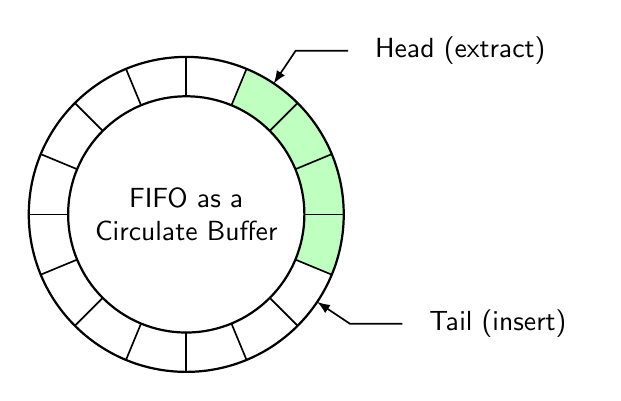
\begin{tikzpicture}[>=latex,font=\sffamily,semithick,scale=2]
			      \fill [green!25] (0,0) -- (67.5:1) arc [end angle=-22.5, start angle=67.5, radius=1] -- cycle;
			      \draw [thick] (0,0) circle (1);
			      \foreach \angle in {90,67.5,...,-67.5}
			      \draw (\angle:1) -- (\angle-180:1);
			      \node [circle,thick,fill=white,draw=black,align=center,minimum size=3cm] at (0,0) {FIFO as a\\Circulate Buffer};
			      \draw [<-] (56.25:1) -- (56.25:1.25) -- +(.333,0)
			      node [right,inner xsep=.333cm] (Head) {Head (extract)};
			      \draw [<-] (-33.75:1) -- (-33.75:1.25) -- +(.333,0)
			      node [right,inner xsep=.333cm] (Tail) {Tail (insert)};
		      \end{tikzpicture}
		      \caption{多缓冲}
	      \end{figure}

	\item 缓冲池:把多个缓冲区连接起来统一管理,既可用于输入又可用于输出的缓冲结构。
\end{enumerate}

\newpage

\section{磁盘调度}

\subsection{磁盘调度算法}

在多道程序系统中,各个进程可能会不断提出不同的对磁盘进行读/写操作的请求。由于有时候这些进程的发送请求的速度比磁盘响应的还要快,因此我们有必要为每个磁盘设备建立一个等待队列。磁盘调度算法的目的就是为了提高磁盘的访问性能,一般是通过优化磁盘的访问请求顺序来做到的。

\begin{figure}[H]
	\centering
	\includegraphics[scale=0.95]{img/C4/4-4/1.png}
	\caption{磁盘}
\end{figure}

假设有下面一个请求序列,每个数字代表磁道的位置:98, 183, 37, 122, 14, 124, 65, 67。初始磁头当前的位置是在第53磁道。

\subsection{先来先服务(FCFS, First Come First Served)}

\begin{figure}[H]
	\centering
	\includegraphics[scale=0.3]{img/C4/4-4/2.png}
	\caption{先来先服务FCFS}
\end{figure}

FCFS算法比较简单粗暴,但是如果大量进程竞争使用磁盘,请求访问的磁道可能会很分散,那FCFS算法因为寻道时间过长,在性能上就会显得很差。

\subsection{最短寻道时间优先(SSTF, Shortest Seek Time First)}

SSTF算法优先选择从当前磁头位置所需寻道时间最短的请求。

\begin{figure}[H]
	\centering
	\includegraphics[scale=0.35]{img/C4/4-4/3.png}
	\caption{最短寻道时间优先SSTF}
\end{figure}

但SSTF算法可能存在某些请求的饥饿,对用户的服务请求的响应机会不是均等的。磁头在一小块区域来回移动,因而导致响应时间的变化幅度很大,有些请求的响应时间将不可预期。

\subsection{扫描算法(SCAN)}

为了防止SSTF算法产生饥饿的问题,可以规定磁头在一个方向上移动,访问所有未完成的请求,直到磁头到达该方向上的最后的磁道,才调换方向。这种算法也叫做电梯调度算法,比如电梯保持按一个方向移动,直到在那个方向上没有请求为止,然后改变方向。

\begin{figure}[H]
	\centering
	\includegraphics[scale=0.35]{img/C4/4-4/3.png}
	\caption{扫描算法SCAN}
\end{figure}

SCAN算法性能较好,不会产生饥饿现象,但是存在这样的问题:中间部分的磁道会比较占便宜,中间部分相比其它部分响应的频率会比较多,也就是说每个磁道的响应频率存在差异。

\subsection{循环扫描算法(CSCAN, Circular Scan)}

CSCAN算法规定只有磁头朝某个特定方向移动时,才处理磁道访问请求,而返回时直接快速移动至最靠边缘的磁道,也就是复位磁头,这个过程是很快的,并且返回中途不处理任何请求。 \\

CSCAN算法的特点就是磁道只响应一个方向上的请求,相比于SCAN算法,对于各个位置磁道响应频率相对比较平均。

\begin{figure}[H]
	\centering
	\includegraphics[scale=1.3]{img/C4/4-4/4.png}
	\caption{循环扫描算法CSCAN}
\end{figure}

\newpage

\section{RAID}

\subsection{RAID(Redundant Array of Independent Disks)}

在单机时代,采用单块磁盘进行数据存储和读写的方式,由于寻址和读写的时间消耗,导致I/O性能非常低,且存储容量还会受到限制。另外,单块磁盘极其容易出现物理故障,经常导致数据的丢失。 \\

1988年美国加州大学伯克利分校的D. A. Patterson教授等首次在论文\textit{A Case of Redundant Array of Inexpensive Disks}中提出了RAID概念,即廉价冗余磁盘阵列(Redundant Array of Inexpensive Disks)。由于当时大容量磁盘比较昂贵,RAID的基本思想是将多个容量较小、相对廉价的磁盘进行有机组合,从而以较低的成本获得与昂贵大容量磁盘相当的容量、性能、可靠性。随着磁盘成本和价格的不断降低,廉价已经毫无意义。因此决定用Independent替代Inexpensive。于时RAID变成了独立磁盘冗余阵列(Redundant Array of Independent Disks),但这仅仅是名称的变化,实质内容没有改变。 \\

RAID思想从提出后就广泛被业界所接纳,存储工业界投入了大量的时间和财力来研究和开发相关产品。随着处理器、内存、计算机接口等技术的不断发展,RAID不断地发展和革新,在计算机存储领域得到了广泛的应用,从高端系统逐渐延伸到普通的中低端系统。 \\

RAID主要优势包括:

\begin{enumerate}
	\item 大容量:扩大了磁盘的容量,由多个磁盘组成的RAID系统具有海量的存储空间。现在单个磁盘的容量就可以到1TB以上,这样RAID的存储容量就可以达到PB级,大多数的存储需求都可以满足。

	\item 高性能:单个磁盘的I/O性能受到接口、带宽等计算机技术的限制,性能往往很有限,容易成为系统性能的瓶颈。通过数据条带化,RAID将数据I/O分散到各个成员磁盘上,从而获得比单个磁盘成倍增长的聚合I/O性能。

	\item 可靠性:RAID冗余技术大幅提升数据可用性和可靠性,保证了若干磁盘出错时,不会导致数据的丢失,不影响系统的连续运行。
\end{enumerate}

\subsection{RAID0}

RAID0是一种简单的、无数据校验的数据条带化技术,将所在磁盘条带化后组成大容量的存储空间,将数据分散存储在所有磁盘中,以独立访问方式实现多块磁盘的并读访问。 \\

RAID0具有低成本、高读写性能,但是它不提供数据冗余保护,一旦数据损坏,将无法恢复。因此,RAID0一般适用于对性能要求严格但对数据安全性和可靠性不高的应用,如视频、音频存储、临时数据缓存空间等。

\begin{figure}[H]
	\centering
	\includegraphics[]{img/C4/4-5/1.png}
\end{figure}

\subsection{RAID1}

RAID1称为镜像,它将数据完全一致地分别写到工作磁盘和镜像磁盘,它的磁盘空间利用率为50\%。RAID1在数据写入时,响应时间会有所影响,但是读数据时没有影响。RAID1提供了最佳的数据保护,一旦工作磁盘发生故障,系统自动从镜像磁盘读取数据。RAID1拥有完全容错的能力,但实现成本高。

\begin{figure}[H]
	\centering
	\includegraphics[]{img/C4/4-5/2.png}
\end{figure}

\subsection{RAID2}

RAID2称为纠错海明码磁盘阵列,其设计思想是利用海明码实现数据校验冗余。海明码是一种在原始数据中加入若干校验码来进行错误检测和纠正的编码技术。海明码自身具备纠错能力,因此RAID2可以在数据发生错误的情况下对纠正错误,保证数据的安全性。 \\

但是海明码的数据冗余开销太大,而且RAID2的数据输出性能受阵列中最慢磁盘驱动器的限制。并且海明码是按位运算,RAID2数据重建非常耗时。因此RAID2在实际中很少应用,没有形成商业产品。

\begin{figure}[H]
	\centering
	\includegraphics[scale=0.5]{img/C4/4-5/3.png}
\end{figure}

\subsection{RAID3}

RAID3是使用专用校验盘的并行访问阵列,它采用一个专用的磁盘作为校验盘,其余磁盘作为数据盘。不同磁盘上同一带区的数据作XOR校验,校验值写入校验盘中。RAID3完好时读性能与RAID0完全一致,并行从多个磁盘条带读取数据,性能非常高,同时还提供了数据容错能力。如果RAID3中某一磁盘出现故障,不会影响数据读取,可以借助校验数据和其他完好数据来重建数据。 \\

RAID3只需要一个校验盘,阵列的存储空间利用率高,再加上并行访问的特征,能够为高带宽的大量读写提供高性能,适用大容量数据的顺序访问应用,如影像处理、流媒体服务等。

\begin{figure}[H]
	\centering
	\includegraphics[]{img/C4/4-5/4.png}
\end{figure}

\subsection{RAID4}

RAID4与RAID3的原理大致相同,区别在于条带化的方式不同。RAID4按照块的方式来组织数据,保证单块的完整性,可以避免受到其他磁盘上同条带产生的不利影响。

\begin{figure}[H]
	\centering
	\includegraphics[]{img/C4/4-5/5.png}
\end{figure}

\subsection{RAID5}

RAID5应该是目前最常见的RAID等级,它的原理与RAID4相似,区别在于校验数据分布在阵列中的所有磁盘上,而没有采用专门的校验磁盘。因此,RAID5不存在RAID4中的并发写操作时的校验盘性能瓶颈问题。 \\

RAID5的磁盘上同时存储数据和校验数据,数据块和对应的校验信息存保存在不同的磁盘上,当一个数据盘损坏时,系统可以根据同一条带的其他数据块和对应的校验数据来重建损坏的数据。 \\

RAID5 兼顾存储性能、数据安全和存储成本等各方面因素,是目前综合性能最佳的数据保护解决方案。RAID5基本上可以满足大部分的存储应用需求,数据中心大多采用它作为应用数据的保护方案。

\begin{figure}[H]
	\centering
	\includegraphics[]{img/C4/4-5/6.png}
\end{figure}

\newpage